% This file was created by tikzplotlib v0.9.8.
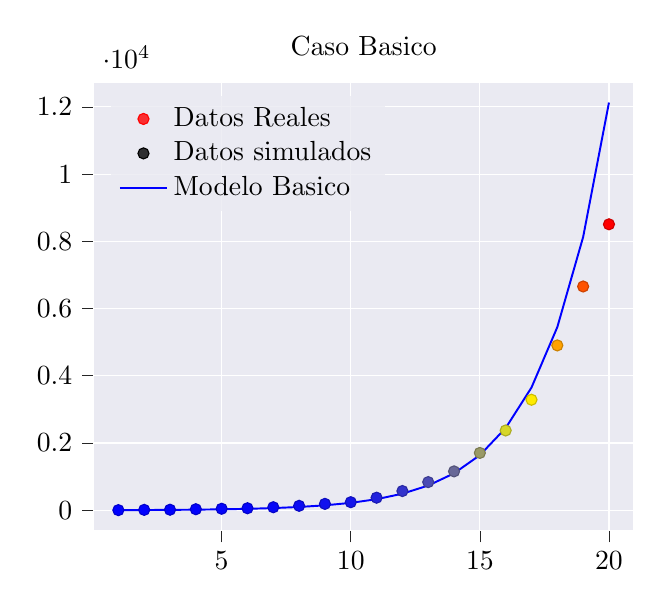
\begin{tikzpicture}

\definecolor{color0}{rgb}{0.917647058823529,0.917647058823529,0.949019607843137}

\begin{axis}[
axis background/.style={fill=color0},
axis line style={white},
legend cell align={left},
legend style={
  fill opacity=0.8,
  draw opacity=1,
  text opacity=1,
  at={(0.03,0.97)},
  anchor=north west,
  draw=none,
  fill=color0
},
tick align=outside,
tick pos=left,
title={Caso Basico},
x grid style={white},
xmajorgrids,
xmin=0.0499999999999999, xmax=20.95,
xtick style={color=white!15!black},
y grid style={white},
ymajorgrids,
ymin=-604.296947802759, ymax=12734.2359038579,
ytick style={color=white!15!black}
]
\addplot [draw=red, fill=red, mark=*, only marks, scatter]
table{%
x  y
1 2
2 10
3 14
4 29
5 43
6 58
7 88
8 130
9 188
10 238
11 372
12 570
13 836
14 1155
15 1704
};
\addlegendentry{Datos Reales}
\addplot [draw=black, fill=black, mark=*, only marks, scatter]
table{%
x  y
16 2372
17 3286
18 4903
19 6656
20 8506
};
\addlegendentry{Datos simulados}
\addplot [line width=0.7pt, blue]
table {%
1 2
2 4.98382139205933
3 9.43541622161865
4 16.0767974853516
5 25.985143661499
6 40.7675094604492
7 62.8214645385742
8 95.7239761352539
9 144.811538696289
10 218.045684814453
11 327.304260253906
12 490.307708740234
13 733.493041992188
14 1096.30102539062
15 1637.57177734375
16 2445.08544921875
17 3649.79223632812
18 5447.03759765625
19 8128.2119140625
20 12127.9384765625
};
\addlegendentry{Modelo Basico}
\end{axis}

\end{tikzpicture}
